% =============================================================================
%  PROYECTO INTEGRADOR DE INFERENCIA ESTADISTICA
%  Entrega final: informe inferencial completo
%
%  Universidad Externado de Colombia
%  Departamento de Matematicas - Pregrado en Ciencia de Datos - 2026-2
%
%  Compilacion:  pdflatex informe_final.tex   (dos veces)
%
%  Ninguna cifra esta escrita a mano: todas provienen de ../salidas/cifras.tex,
%  que genera el script analisis_final.R. Si la base cambia, basta con volver
%  a correr el script y recompilar.
% =============================================================================

\documentclass[12pt,letterpaper]{article}
% =============================================================================
%  Preambulo comun - Formato APA 7 (estudiante)
%  Times New Roman 12 pt, texto negro, margenes de 1 pulgada, interlineado
%  doble, sangria de primera linea de media pulgada y numeracion superior
%  derecha, conforme a APA (2020, secciones 2.19 a 2.24).
% =============================================================================

\usepackage[utf8]{inputenc}
\usepackage[T1]{fontenc}
\usepackage[spanish,es-nodecimaldot,es-tabla]{babel}
\usepackage{mathptmx}          % Times New Roman (texto y matematicas)
\usepackage[letterpaper,margin=1in]{geometry}
\usepackage{setspace}
\usepackage{graphicx}
\usepackage{array}
\usepackage{amsmath}
\usepackage{titlesec}
\usepackage{fancyhdr}
\usepackage{enumitem}
\usepackage{xcolor}
\usepackage{float}
\usepackage[hidelinks]{hyperref}

% --- Color del texto: negro en todo el documento ---------------------------
\color{black}
\definecolor{negro}{gray}{0}

% --- Alineacion --------------------------------------------------------------
% El documento sale JUSTIFICADO, que es la convencion habitual en los trabajos
% academicos en espanol. APA 7 (seccion 2.24) prescribe, en rigor, alineacion a
% la izquierda con margen derecho irregular: para adoptarla basta con quitar el
% comentario de las dos lineas siguientes.
% \usepackage[document]{ragged2e}
% \setlength{\RaggedRightParindent}{0.5in}

% --- Interlineado y sangria --------------------------------------------------
% Interlineado doble y sangria de primera linea de media pulgada en todo el
% cuerpo, salvo en las tablas, las figuras y sus notas.
\doublespacing
\setlength{\parindent}{0.5in}
\setlength{\parskip}{0pt}
% Holgura extra para que el texto justificado no se salga del margen
\setlength{\emergencystretch}{1.5em}
% Particion correcta de palabras inglesas de las referencias
\hyphenation{mis-in-ter-pre-ta-tions ho-mo-sce-das-tic-i-ty}

% --- Numeracion de pagina: superior derecha ---------------------------------
\setlength{\headheight}{14.5pt}
\pagestyle{fancy}
\fancyhf{}
\fancyhead[R]{\normalfont\normalsize\thepage}
\renewcommand{\headrulewidth}{0pt}

% --- Niveles de titulo APA 7 -------------------------------------------------
% Nivel 1: centrado, negrita.  Nivel 2: izquierda, negrita.
% Nivel 3: izquierda, negrita cursiva.
\titleformat{\section}{\normalsize\bfseries\centering}{}{0pt}{}
\titleformat{\subsection}{\normalsize\bfseries\raggedright}{}{0pt}{}
\titleformat{\subsubsection}{\normalsize\bfseries\itshape\raggedright}{}{0pt}{}
\titlespacing*{\section}{0pt}{0pt}{0pt}
\titlespacing*{\subsection}{0pt}{0pt}{0pt}
\titlespacing*{\subsubsection}{0pt}{0pt}{0pt}
\setcounter{secnumdepth}{0}

% --- Encabezados de tabla y figura al estilo APA -----------------------------
% Numero en negrita, en linea propia; titulo en cursiva, en la linea siguiente.
\newcommand{\apatabla}[2]{%
  \noindent{\normalsize\textbf{Tabla #1}}\par
  \noindent{\normalsize\textit{#2}}\par
  \vspace{4pt}}

\newcommand{\apafigura}[2]{%
  \noindent{\normalsize\textbf{Figura #1}}\par
  \noindent{\normalsize\textit{#2}}\par
  \vspace{4pt}}

% Nota de tabla o figura, a espacio sencillo. Se usa un grupo con
% \setstretch{1} y no el entorno spacing de setspace: ese entorno, al cerrarse
% dentro de un documento a doble espacio, inserta un salto negativo que monta
% el texto siguiente sobre la tabla.
\newcommand{\apanota}[1]{%
  \par\vspace{4pt}%
  \begingroup\setstretch{1}\footnotesize
  \noindent\textit{Nota.} #1\par
  \endgroup}

% --- Entorno de referencias con sangria francesa -----------------------------
\newenvironment{referencias}
  {\begin{list}{}{%
     \setlength{\leftmargin}{0.5in}
     \setlength{\itemindent}{-0.5in}
     \setlength{\listparindent}{0pt}
     \setlength{\labelwidth}{0pt}
     \setlength{\labelsep}{0pt}
     \setlength{\itemsep}{0pt}
     \setlength{\parsep}{0pt}
     \setlength{\topsep}{0pt}}}
  {\end{list}}

% --- Espaciado sencillo dentro de tablas y figuras ---------------------------
\newenvironment{apacuerpo}{\par\begingroup\setstretch{1}}{\par\endgroup}

% --- Bloque indivisible: encabezado, tabla o figura y nota en la misma pagina
\newenvironment{bloque}{\par\noindent\begin{minipage}{\linewidth}}%
  {\end{minipage}\par}

\newcommand{\Ndescargados}{28.663}
\newcommand{\Nmaiz}{21.992}
\newcommand{\Nfinal}{19.826}
\newcommand{\Nmunicipios}{1.043}
\newcommand{\Ndepartamentos}{32}
\newcommand{\AnioMin}{2019}
\newcommand{\AnioMax}{2025}
\newcommand{\NTrad}{15.935}
\newcommand{\NTec}{3.891}
\newcommand{\PctTec}{19{,}6}
\newcommand{\Alfa}{0{,}05}
\newcommand{\NivelConf}{95}
\newcommand{\MediaTrad}{1{,}85}
\newcommand{\MediaTec}{4{,}37}
\newcommand{\MedianaTrad}{1{,}50}
\newcommand{\MedianaTec}{4{,}50}
\newcommand{\DETrad}{1{,}25}
\newcommand{\DETec}{1{,}96}
\newcommand{\AsimTrad}{4{,}34}
\newcommand{\AsimTec}{1{,}92}
\newcommand{\QITrad}{1{,}12}
\newcommand{\QIIITrad}{2{,}00}
\newcommand{\QITec}{3{,}00}
\newcommand{\QIIITec}{5{,}20}
\newcommand{\RazonMedias}{2{,}36}
\newcommand{\VTF}{2{,}46}
\newcommand{\VTglUno}{3.890}
\newcommand{\VTglDos}{15.934}
\newcommand{\VTp}{\ensuremath{<}\,0{,}001}
\newcommand{\VTpRel}{\ensuremath{<}~0{,}001}
\newcommand{\VTcritInf}{0{,}951}
\newcommand{\VTcritSup}{1{,}050}
\newcommand{\VTicInf}{2{,}34}
\newcommand{\VTicSup}{2{,}59}
\newcommand{\WDif}{2{,}52}
\newcommand{\WEE}{0{,}033}
\newcommand{\Wt}{76{,}43}
\newcommand{\Wgl}{4.688{,}6}
\newcommand{\Wcrit}{1{,}960}
\newcommand{\Wp}{\ensuremath{<}\,0{,}001}
\newcommand{\WpRel}{\ensuremath{<}~0{,}001}
\newcommand{\WicInf}{2{,}45}
\newcommand{\WicSup}{2{,}58}
\newcommand{\NPares}{2.808}
\newcommand{\NMunPares}{211}
\newcommand{\PDif}{2{,}36}
\newcommand{\PDE}{1{,}74}
\newcommand{\Pt}{72{,}14}
\newcommand{\Pgl}{2.807}
\newcommand{\Pcrit}{1{,}961}
\newcommand{\Pp}{\ensuremath{<}\,0{,}001}
\newcommand{\PpRel}{\ensuremath{<}~0{,}001}
\newcommand{\PicInf}{2{,}30}
\newcommand{\PicSup}{2{,}43}
\newcommand{\PPctTecMayor}{94{,}6}
\newcommand{\MNTec}{261}
\newcommand{\MNTrad}{1.007}
\newcommand{\MDif}{2{,}33}
\newcommand{\Mt}{21{,}42}
\newcommand{\Mgl}{288{,}5}
\newcommand{\Mcrit}{1{,}968}
\newcommand{\Mp}{\ensuremath{<}\,0{,}001}
\newcommand{\MpRel}{\ensuremath{<}~0{,}001}
\newcommand{\MicInf}{2{,}11}
\newcommand{\MicSup}{2{,}54}
\newcommand{\CorteRend}{15{,}0}
\newcommand{\NExcluRend}{17}
\newcommand{\RDif}{2{,}50}
\newcommand{\RicInf}{2{,}44}
\newcommand{\RicSup}{2{,}56}
\newcommand{\XTrad}{6.909}
\newcommand{\XTec}{1.345}
\newcommand{\PropTrad}{43{,}4}
\newcommand{\PropTec}{34{,}6}
\newcommand{\PropComb}{41{,}6}
\newcommand{\ICTradInf}{42{,}6}
\newcommand{\ICTradSup}{44{,}1}
\newcommand{\ICTecInf}{33{,}1}
\newcommand{\ICTecSup}{36{,}1}
\newcommand{\CondNp}{1.345}
\newcommand{\Zp}{9{,}97}
\newcommand{\ZChi}{99{,}45}
\newcommand{\Zcrit}{1{,}96}
\newcommand{\ZpVal}{\ensuremath{<}\,0{,}001}
\newcommand{\ZpRel}{\ensuremath{<}~0{,}001}
\newcommand{\DifProp}{8{,}8}
\newcommand{\DifPropInf}{7{,}1}
\newcommand{\DifPropSup}{10{,}5}
\newcommand{\RazonProp}{1{,}25}
\newcommand{\PctCosMayor}{17{,}5}
\newcommand{\NAnualTrad}{8.781}
\newcommand{\NAnualTec}{2.193}
\newcommand{\PropAnualTrad}{46{,}9}
\newcommand{\PropAnualTec}{37{,}4}
\newcommand{\DifPropAnual}{9{,}5}
\newcommand{\ZAnual}{8{,}01}
\newcommand{\ZAnualP}{\ensuremath{<}\,0{,}001}
\newcommand{\ZAnualPRel}{\ensuremath{<}~0{,}001}
\newcommand{\DifPropAnualInf}{7{,}2}
\newcommand{\DifPropAnualSup}{11{,}8}
\newcommand{\RGN}{19.826}
\newcommand{\RGIntEst}{\ensuremath{-}93{,}99}
\newcommand{\RGIntEE}{13{,}13}
\newcommand{\RGIntT}{\ensuremath{-}7{,}16}
\newcommand{\RGIntP}{\ensuremath{<}\,0{,}001}
\newcommand{\RGIntPRel}{\ensuremath{<}~0{,}001}
\newcommand{\RGIntLi}{\ensuremath{-}119{,}72}
\newcommand{\RGIntLs}{\ensuremath{-}68{,}26}
\newcommand{\RGPenEst}{3{,}60}
\newcommand{\RGPenEE}{0{,}0144}
\newcommand{\RGPenT}{250{,}32}
\newcommand{\RGPenP}{\ensuremath{<}\,0{,}001}
\newcommand{\RGPenPRel}{\ensuremath{<}~0{,}001}
\newcommand{\RGPenLi}{3{,}58}
\newcommand{\RGPenLs}{3{,}63}
\newcommand{\RGRdos}{0{,}760}
\newcommand{\RGRdosAj}{0{,}760}
\newcommand{\RGRdosPct}{76}
\newcommand{\RGF}{62.658{,}8}
\newcommand{\RGglNum}{1}
\newcommand{\RGglDen}{19.824}
\newcommand{\RGpF}{\ensuremath{<}\,0{,}001}
\newcommand{\RGpFRel}{\ensuremath{<}~0{,}001}
\newcommand{\RGSigma}{1.810{,}2}
\newcommand{\RGTcrit}{1{,}960}
\newcommand{\RGFcrit}{3{,}842}
\newcommand{\RTradN}{15.935}
\newcommand{\RTradIntEst}{9{,}150}
\newcommand{\RTradIntEE}{3{,}565}
\newcommand{\RTradIntT}{2{,}57}
\newcommand{\RTradIntP}{0{,}010}
\newcommand{\RTradIntPRel}{\ensuremath{=}~0{,}010}
\newcommand{\RTradIntLi}{2{,}162}
\newcommand{\RTradIntLs}{16{,}139}
\newcommand{\RTradPenEst}{1{,}83}
\newcommand{\RTradPenEE}{0{,}0106}
\newcommand{\RTradPenT}{172{,}01}
\newcommand{\RTradPenP}{\ensuremath{<}\,0{,}001}
\newcommand{\RTradPenPRel}{\ensuremath{<}~0{,}001}
\newcommand{\RTradPenLi}{1{,}81}
\newcommand{\RTradPenLs}{1{,}85}
\newcommand{\RTradRdos}{0{,}650}
\newcommand{\RTradRdosAj}{0{,}650}
\newcommand{\RTradRdosPct}{65}
\newcommand{\RTradF}{29.587{,}7}
\newcommand{\RTradglNum}{1}
\newcommand{\RTradglDen}{15.933}
\newcommand{\RTradpF}{\ensuremath{<}\,0{,}001}
\newcommand{\RTradpFRel}{\ensuremath{<}~0{,}001}
\newcommand{\RTradSigma}{410{,}3}
\newcommand{\RTradTcrit}{1{,}960}
\newcommand{\RTradFcrit}{3{,}842}
\newcommand{\RTecN}{3.891}
\newcommand{\RTecIntEst}{428{,}05}
\newcommand{\RTecIntEE}{61{,}81}
\newcommand{\RTecIntT}{6{,}93}
\newcommand{\RTecIntP}{\ensuremath{<}\,0{,}001}
\newcommand{\RTecIntPRel}{\ensuremath{<}~0{,}001}
\newcommand{\RTecIntLi}{306{,}87}
\newcommand{\RTecIntLs}{549{,}24}
\newcommand{\RTecPenEst}{3{,}75}
\newcommand{\RTecPenEE}{0{,}0318}
\newcommand{\RTecPenT}{117{,}97}
\newcommand{\RTecPenP}{\ensuremath{<}\,0{,}001}
\newcommand{\RTecPenPRel}{\ensuremath{<}~0{,}001}
\newcommand{\RTecPenLi}{3{,}69}
\newcommand{\RTecPenLs}{3{,}82}
\newcommand{\RTecRdos}{0{,}782}
\newcommand{\RTecRdosAj}{0{,}782}
\newcommand{\RTecRdosPct}{78}
\newcommand{\RTecF}{13.918{,}0}
\newcommand{\RTecglNum}{1}
\newcommand{\RTecglDen}{3.889}
\newcommand{\RTecpF}{\ensuremath{<}\,0{,}001}
\newcommand{\RTecpFRel}{\ensuremath{<}~0{,}001}
\newcommand{\RTecSigma}{3.783{,}9}
\newcommand{\RTecTcrit}{1{,}961}
\newcommand{\RTecFcrit}{3{,}844}
\newcommand{\RGBootLi}{2{,}89}
\newcommand{\RGBootLs}{4{,}95}
\newcommand{\RGBootSE}{0{,}540}
\newcommand{\RGBootRazonAncho}{37}
\newcommand{\RTradBootLi}{1{,}72}
\newcommand{\RTradBootLs}{1{,}94}
\newcommand{\RTradBootSE}{0{,}056}
\newcommand{\RTradBootRazonAncho}{5}
\newcommand{\RTecBootLi}{2{,}91}
\newcommand{\RTecBootLs}{5{,}49}
\newcommand{\RTecBootSE}{0{,}687}
\newcommand{\RTecBootRazonAncho}{21}
\newcommand{\BBoot}{2.000}
\newcommand{\CorrArea}{0{,}87}
\newcommand{\MediaRendGlobal}{2{,}34}
\newcommand{\RGSWW}{0{,}18}
\newcommand{\RGSWp}{\ensuremath{<}\,0{,}001}
\newcommand{\RGSWpRel}{\ensuremath{<}~0{,}001}
\newcommand{\RGSWn}{5.000}
\newcommand{\RGDERazon}{18}
\newcommand{\RTradSWW}{0{,}44}
\newcommand{\RTradSWp}{\ensuremath{<}\,0{,}001}
\newcommand{\RTradSWpRel}{\ensuremath{<}~0{,}001}
\newcommand{\RTradSWn}{5.000}
\newcommand{\RTradDERazon}{24}
\newcommand{\RTecSWW}{0{,}23}
\newcommand{\RTecSWp}{\ensuremath{<}\,0{,}001}
\newcommand{\RTecSWpRel}{\ensuremath{<}~0{,}001}
\newcommand{\RTecSWn}{3.891}
\newcommand{\RTecDERazon}{16}
\newcommand{\RGPenSinGrandes}{2{,}85}
\newcommand{\RGRdosSinGrandes}{0{,}39}
\newcommand{\CorteArea}{1.992}
\newcommand{\NGrandes}{199}
\newcommand{\PctTecGrandes}{57}
\newcommand{\PctTecTotal}{20}
\newcommand{\DecVT}{Se rechaza}
\newcommand{\DecW}{Se rechaza}
\newcommand{\DecP}{Se rechaza}
\newcommand{\DecM}{Se rechaza}
\newcommand{\DecZ}{Se rechaza}
\newcommand{\DecZA}{Se rechaza}
\newcommand{\DecRG}{Se rechaza}
\newcommand{\DecRTrad}{Se rechaza}
\newcommand{\DecRTec}{Se rechaza}
\newcommand{\BrechaMinIC}{2{,}11}
\newcommand{\BrechaMaxIC}{2{,}58}
\newcommand{\Nexcluidos}{2.166}
\newcommand{\VersionR}{R version 4.6.1 (2026-06-24 ucrt)}
\newcommand{\VersionRCorta}{R 4.6.1}
\newcommand{\Semilla}{20261117}


% Columna de parrafo alineada a la izquierda, para las tablas
\newcolumntype{L}[1]{>{\raggedright\arraybackslash}p{#1}}

\begin{document}

% =============================================================================
%  Portada - APA 7, formato para trabajo de estudiante (seccion 2.3)
% =============================================================================
\thispagestyle{fancy}
\begin{center}
\vspace*{3cm}

{\bfseries Rendimiento, pérdida de área y escala en el cultivo de maíz\\[2pt]
en Colombia, 2019--2025: un análisis inferencial}

\vspace{1.2cm}

Santiago Bernal, Santiago Parra, Daniel Núñez y Andrés Felipe Baquero

\vspace{0.7cm}

Departamento de Matemáticas, Universidad Externado de Colombia

\vspace{0.7cm}

Pregrado en Ciencia de Datos

\vspace{0.7cm}

Inferencia Estadística

\vspace{0.7cm}

Proyecto integrador --- Entrega final

\vspace{0.7cm}

Noviembre de 2026

\end{center}
\newpage


% =============================================================================
%  CUERPO DEL INFORME  (extension exigida: 3 a 5 paginas)
% =============================================================================

\begin{center}
\textbf{Rendimiento, pérdida de área y escala en el cultivo de maíz\\[2pt]
en Colombia, 2019--2025: un análisis inferencial}
\end{center}

En la Entrega~1 se describieron los registros de maíz de las Evaluaciones
Agropecuarias Municipales y se plantearon tres preguntas: si el rendimiento
medio difiere entre el maíz tecnificado y el tradicional, si la proporción de
registros con pérdida de área difiere entre ambos sistemas y cómo se relaciona
el área sembrada con la producción. Este informe las responde con las
herramientas inferenciales del curso: dos comparaciones de grupos,
complementadas con una prueba pareada, y regresiones lineales simples con
diagnóstico de residuos (Universidad Externado de Colombia, 2026).

\section{Datos y marco inferencial}

Se emplea la base de la Entrega~1, publicada por la Unidad de Planificación de
Tierras Rurales, Adecuación de Tierras y Usos Agropecuarios [UPRA] (2025), con
la misma depuración. De los \Nmaiz{} registros de maíz se conservan los
\Nfinal{} que tienen área sembrada, producción y rendimiento positivos; cubren
\Nmunicipios{} municipios de \Ndepartamentos{} departamentos entre \AnioMin{}
y \AnioMax. Cada registro es la evaluación de una desagregación de maíz en un
municipio durante un semestre: \NTrad{} corresponden al sistema tradicional y
\NTec{} al tecnificado. La Tabla~1 resume las variables que intervienen en los
contrastes.

Como las evaluaciones cubren casi todos los municipios productores, la
inferencia no se refiere a la lista finita de registros sino al proceso que
los genera: el resultado de cada temporada depende del clima, las plagas y el
manejo, y los registros de \AnioMin{} a \AnioMax{} se tratan como una muestra
de ese proceso. La Tabla~2 formula el parámetro y las hipótesis de cada
pregunta. Todos los contrastes son bilaterales, con un nivel de significancia
$\alpha = \Alfa$, y cada estadístico obtenido con las funciones de R se
verificó a mano con su distribución de referencia.

\section{Comparación de grupos}

\subsection{Rendimiento medio según el sistema de producción}

La Figura~1 muestra la diferencia que motiva la primera pregunta: la mitad
central de los registros tecnificados, entre \QITec{} y \QIIITec{} t/ha,
queda por completo por encima de la mitad central de los tradicionales, entre
\QITrad{} y \QIIITrad{} t/ha, y las medias son \MediaTec{} y \MediaTrad{} t/ha,
respectivamente. Ambas
distribuciones son asimétricas (coeficientes de \AsimTec{} y \AsimTrad), pero
con \NTec{} y \NTrad{} registros el teorema del límite central respalda la
normalidad aproximada de las medias muestrales, que es lo que exige la
prueba~\textit{t}. La prueba~\textit{F} rechazó la igualdad de varianzas
($F = \VTF$, $p$~\VTpRel): la varianza del sistema tecnificado es \VTF{} veces
la del tradicional, por lo que se aplicó la corrección de Welch (Wackerly et
al., 2010).

La Tabla~3 reúne los resultados. El rendimiento medio del maíz tecnificado
supera al del tradicional en \WDif{} t/ha ($t(\Wgl) = \Wt$, $p$~\WpRel;
IC~95\,\%: [\WicInf; \WicSup]). Se rechaza $H_0$: con un 95\,\% de confianza,
la brecha poblacional está entre \WicInf{} y \WicSup{} t/ha, de modo que el
sistema tecnificado rinde en promedio \RazonMedias{} veces lo que rinde el
tradicional. Es una diferencia de gran relevancia práctica, mayor que el
propio rendimiento medio del sistema tradicional.

Como el maíz tecnificado se siembra en otras zonas, la brecha podría reflejar
el lugar y no el sistema. Para controlarlo se formaron \NPares{} pares en los
que un mismo municipio reportó ambos sistemas en el mismo año, semestre y
color de grano (\NMunPares{} municipios). Dentro de esos pares, la diferencia
media fue de \PDif{} t/ha ($t(\Pgl) = \Pt$, $p$~\PpRel; IC~95\,\%: [\PicInf;
\PicSup]) y el tecnificado rindió más en el \PPctTecMayor\,\% de los casos. La
Figura~2 compara esta estimación con la de Welch y con una tercera que reduce
cada municipio a un promedio por sistema, para que los municipios con muchos
registros no pesen más: los tres intervalos excluyen el cero y ubican la
brecha entre \BrechaMinIC{} y \BrechaMaxIC{} t/ha.

\subsection{Pérdida de área según el sistema de producción}

Un registro tiene pérdida de área cuando el área cosechada es menor que la
sembrada. La reportan \XTrad{} de los \NTrad{} registros tradicionales
(\PropTrad\,\%) y \XTec{} de los \NTec{} tecnificados (\PropTec\,\%); como cada
grupo tiene al menos \CondNp{} éxitos y fracasos, la aproximación normal es
adecuada. La prueba~\textit{Z} para dos proporciones rechaza la igualdad
($Z = \Zp$, $p$~\ZpRel; IC~95\,\% para la diferencia: [\DifPropInf;
\DifPropSup] puntos porcentuales). La Figura~3 lo hace visible: los intervalos
de los dos sistemas no se tocan y la pérdida es \RazonProp{} veces más
frecuente en el sistema tradicional.

El indicador tiene una limitación de medición: en el \PctCosMayor\,\% de los
registros el área cosechada supera a la sembrada, lo que indica que parte de
lo sembrado en un semestre se cosecha en el siguiente. Para atenuar ese desfase, el
contraste se repitió con el total anual de cada municipio y desagregación; la
brecha se mantuvo (\PropAnualTrad\,\% frente a \PropAnualTec\,\%; IC~95\,\%:
[\DifPropAnualInf; \DifPropAnualSup] puntos), de modo que la conclusión no
depende del calendario de cosecha.

\section{Relación entre el área sembrada y la producción}

El modelo planteado en la Entrega~1 es
\[
\text{producción}_i = \beta_0 + \beta_1\,\text{área}_i + \varepsilon_i ,
\]
y se ajustó con todos los registros y, por separado, dentro de cada sistema
(Tabla~4). La Figura~4 muestra una relación creciente (correlación de Pearson
de \CorrArea), con la mayoría de los registros en áreas pequeñas y unos pocos
registros muy grandes. Con todos los registros, cada hectárea sembrada
adicional se asocia, en promedio, con \RGPenEst{} toneladas más de producción
($t(\RGglDen) = \RGPenT$, $p$~\RGPenPRel; IC~95\,\%: [\RGPenLi; \RGPenLs]).
La prueba~\textit{F} global ($F = \RGF$, $p$~\RGpFRel), que en la regresión
simple es el cuadrado de~\textit{t}, lleva a la misma conclusión: se rechaza
$H_0\colon \beta_1 = 0$. El área explica el \RGRdosPct\,\% de la variabilidad
de la producción ($R^2 = \RGRdos$; $R^2$~ajustado $= \RGRdosAj$). El
intercepto (\RGIntEst~t; $t = \RGIntT$, $p$~\RGIntPRel) no tiene lectura
práctica: corresponde a un área de cero hectáreas y daría una producción
negativa.

El diagnóstico de residuos (Figura~5 y Tabla~5) muestra que los supuestos no
se cumplen. En el gráfico de residuos frente a valores ajustados, la
dispersión se abre a medida que crece el valor ajustado: la desviación
estándar de los residuos en el tercio de valores ajustados más altos es
\RGDERazon{} veces la del tercio más bajo, así que la varianza no es
constante. Además, en la mayoría de los registros los residuos bajan cuando
crece el valor ajustado, señal de que la recta la inclinan los registros más
grandes: sin el 1\,\% de áreas mayores (más de \CorteArea{}~ha), la pendiente
baja a \RGPenSinGrandes{} y el $R^2$ a \RGRdosSinGrandes. El gráfico
cuantil-cuantil muestra colas mucho más pesadas que las de la normal, y la
prueba de Shapiro-Wilk rechaza la normalidad de los errores ($W = \RGSWW$,
$p$~\RGSWpRel; se aplicó a una muestra aleatoria de \RGSWn{} residuos, el
máximo que admite la función). La independencia tampoco está garantizada: un
mismo municipio aporta registros de varios semestres, que comparten suelo,
clima y productores. Con estas violaciones, el error estándar y el intervalo
clásicos de la pendiente no son confiables.

Por eso el intervalo de la pendiente se recalculó con bootstrap percentil: se
remuestrearon los registros \BBoot{} veces, se volvió a ajustar la recta en
cada remuestreo y se tomaron los percentiles 2,5 y 97,5 de las pendientes
obtenidas (Efron y Tibshirani, 1993). Este intervalo no exige normalidad ni
varianza constante. El resultado, [\RGBootLi; \RGBootLs] t/ha, es unas
\RGBootRazonAncho{} veces más ancho que el clásico, pero sigue sin incluir el
cero: la relación positiva se mantiene, aunque su magnitud es bastante más
incierta de lo que indica el intervalo clásico.

La pendiente tiene una lectura directa: es la producción adicional por
hectárea sembrada, es decir, un rendimiento. La Figura~6 compara las tres
estimaciones. Dentro del sistema tradicional, la pendiente es de
\RTradPenEst{} t/ha (IC bootstrap: [\RTradBootLi; \RTradBootLs]) y dentro del
tecnificado, de \RTecPenEst{} t/ha ([\RTecBootLi; \RTecBootLs]); los
intervalos no se cruzan, y los rendimientos medios de la primera pregunta
(\MediaTrad{} y \MediaTec{} t/ha) caen dentro de ellos. La pendiente con todos
los registros queda cerca de la del tecnificado, y por encima del rendimiento
medio de la base (\MediaRendGlobal{} t/ha), porque los registros de mayor área,
que son los que más pesan en la recta, son tecnificados en un
\PctTecGrandes\,\%, frente al \PctTecTotal\,\% de toda la base. Los residuos de
los dos modelos por sistema muestran el mismo patrón (Tabla~5), por lo que
también para ellos se reporta el intervalo bootstrap.

\section{Conclusiones}

Primera pregunta: el rendimiento medio del maíz tecnificado supera al del
tradicional en \WDif{} t/ha (IC~95\,\%: [\WicInf; \WicSup]), y la brecha
persiste al comparar ambos sistemas dentro del mismo municipio y semestre.
Segunda: la pérdida de área es más frecuente en el sistema tradicional, con
\DifProp{} puntos porcentuales de diferencia (IC~95\,\%: [\DifPropInf;
\DifPropSup]). Tercera: la producción aumenta con el área sembrada; cada
hectárea adicional se asocia, en promedio, con \RGPenEst{} t más (IC bootstrap
95\,\%: [\RGBootLi; \RGBootLs]), y el área explica el \RGRdosPct\,\% de la
variabilidad de la producción. Como el modelo no cumple los supuestos de
normalidad ni de varianza constante, la incertidumbre se midió con bootstrap,
y la relación sigue siendo significativa. Esa pendiente es un rendimiento, y
es mayor en el sistema tecnificado que en el tradicional (\RTecPenEst{} frente
a \RTradPenEst{} t/ha), lo que concuerda con la primera pregunta.

El alcance tiene cuatro límites. Los datos son observacionales: el sistema
tecnificado suele ir acompañado de semilla mejorada, crédito y productores de
mayor escala, y aunque la comparación pareada controla el lugar y la
temporada, no controla esos factores; las brechas son asociaciones, no el efecto causal
de tecnificar. Los registros de un mismo municipio no son independientes, lo
que estrecha los intervalos; en las comparaciones de grupos, las
verificaciones con un promedio por municipio y con totales anuales muestran
que las conclusiones se sostienen, pero en la regresión ni el intervalo
clásico ni el bootstrap, que remuestrea registros, corrigen esa dependencia. El
indicador de pérdida mezcla pérdidas reales con el calendario de cosecha, y
las cifras de la EVA provienen de evaluaciones de los técnicos municipales,
no de mediciones directas en cada predio. Por último, con casi veinte mil registros incluso diferencias
pequeñas resultan significativas; por eso se reportaron siempre la magnitud y
su intervalo, y se distinguió la significancia estadística de la relevancia
práctica (Greenland et al., 2016).

\subsection{Nota sobre herramientas y reproducibilidad}

El análisis se realizó en \VersionRCorta{} solo con funciones vistas en clase:
\texttt{var.test}, \texttt{t.test}, \texttt{prop.test}, \texttt{lm},
\texttt{confint}, \texttt{anova}, \texttt{shapiro.test}, y \texttt{boot} y
\texttt{boot.ci} del paquete \texttt{boot} (R Core Team, 2026). El script
\texttt{analisis\_final.R} reproduce las tablas, las figuras y cada cifra del
texto. Se usó Claude (Anthropic, 2026) como apoyo en la depuración del código
y en la edición del documento; el diseño del análisis, la verificación de los
resultados y las conclusiones son responsabilidad de los autores.

\newpage

% =============================================================================
%  REFERENCIAS
% =============================================================================

\section{Referencias}
\vspace{6pt}

\begin{referencias}

\item Anthropic. (2026). \textit{Claude} [Modelo de lenguaje de gran escala]. \url{https://claude.ai}

\item Efron, B., \& Tibshirani, R. J. (1993). \textit{An introduction to the bootstrap}. Chapman \& Hall/CRC.

\item Greenland, S., Senn, S. J., Rothman, K. J., Carlin, J. B., Poole, C., Goodman, S. N., \& Altman, D. G. (2016). Statistical tests, \textit{P} values, confidence intervals, and power: A guide to misinterpretations. \textit{European Journal of Epidemiology}, \textit{31}(4), 337--350. \url{https://doi.org/10.1007/s10654-016-0149-3}

\item R Core Team. (2026). \textit{R: A language and environment for statistical computing} (Versión 4.6.1) [Software]. R Foundation for Statistical Computing. \url{https://www.R-project.org/}

\item Unidad de Planificación de Tierras Rurales, Adecuación de Tierras y Usos Agropecuarios. (2025). \textit{Evaluaciones Agropecuarias Municipales --- EVA. 2019--2025. Base agrícola} [Conjunto de datos]. Datos Abiertos Colombia. Recuperado el 6 de noviembre de 2026, de \url{https://www.datos.gov.co/d/uejq-wxrr}

\item Universidad Externado de Colombia. (2026). \textit{Guía del proyecto: Asignatura Inferencia Estadística} [Documento de curso].

\item Wackerly, D. D., Mendenhall, W., \& Scheaffer, R. L. (2010). \textit{Estadística matemática con aplicaciones} (7.\textsuperscript{a} ed.). Cengage Learning.

\end{referencias}


\newpage

% =============================================================================
%  TABLAS Y FIGURAS (formato de manuscrito APA; no cuentan en la extension)
% =============================================================================

\section{Tablas}
\vspace{6pt}

\begin{bloque}
\apatabla{1}{Variables que intervienen en los contrastes}

\begin{apacuerpo}
\noindent\footnotesize
\setlength{\tabcolsep}{4pt}
\begin{tabular}{@{}L{3.1cm} L{6.0cm} L{2.6cm} L{3.9cm}@{}}
\hline
\textbf{Variable} & \textbf{Descripción} & \textbf{Tipo} & \textbf{Uso en el análisis} \\
\hline
\texttt{rendimiento} & Toneladas obtenidas por hectárea cosechada. & Numérica continua & Respuesta de la pregunta~1. \\
\texttt{sistema} & Tradicional o tecnificado, según la desagregación del cultivo. & Categórica binaria & Define los grupos de las preguntas~1 y~2 y separa los modelos de la pregunta~3. \\
\texttt{area\_sembrada} & Hectáreas sembradas en el semestre. & Numérica continua & Explicativa de la pregunta~3; define la pérdida. \\
\texttt{area\_cosechada} & Hectáreas cosechadas en el semestre. & Numérica continua & Define la pérdida. \\
\texttt{perdida} & Verdadero si el área cosechada es menor que la sembrada. & Categórica binaria & Respuesta de la pregunta~2. \\
\texttt{produccion} & Toneladas obtenidas en el semestre. & Numérica continua & Respuesta de la pregunta~3. \\
\texttt{municipio}, \texttt{anio}, \texttt{periodo}, \texttt{color} & Código DANE del municipio, año, semestre (A o B) y color del grano. & Categóricas & Forman los pares de la comparación pareada. \\
\hline
\end{tabular}
\end{apacuerpo}

\apanota{$N = \Nfinal$ registros de maíz. \texttt{sistema}, \texttt{perdida}
y \texttt{color} son variables derivadas en el script; las demás provienen de
UPRA (2025). El diccionario completo se presentó en la Entrega~1.}
\end{bloque}

\vspace{14pt}

\begin{bloque}
\apatabla{2}{Planteamiento formal de las hipótesis}

\begin{apacuerpo}
\noindent\footnotesize
\setlength{\tabcolsep}{4pt}
\begin{tabular}{@{}L{2.5cm} L{4.3cm} L{4.5cm} L{4.3cm}@{}}
\hline
\textbf{Pregunta} & \textbf{Parámetro} & \textbf{Hipótesis} & \textbf{Contraste} \\
\hline
1. Rendimiento & $\mu_{\text{tec}} - \mu_{\text{trad}}$: diferencia de rendimientos medios (t/ha). & $H_0\colon \mu_{\text{tec}} - \mu_{\text{trad}} = 0$ \newline $H_1\colon \mu_{\text{tec}} - \mu_{\text{trad}} \neq 0$ & \textit{t} de Welch para muestras independientes. \\
1. Supuesto previo & $\sigma^2_{\text{tec}} / \sigma^2_{\text{trad}}$: razón de varianzas. & $H_0\colon \sigma^2_{\text{tec}} / \sigma^2_{\text{trad}} = 1$ \newline $H_1\colon \sigma^2_{\text{tec}} / \sigma^2_{\text{trad}} \neq 1$ & \textit{F} para dos varianzas. \\
1. Complemento & $\mu_D$: media de $D$ = rendimiento tecnificado menos tradicional en el mismo municipio, año, semestre y color. & $H_0\colon \mu_D = 0$ \newline $H_1\colon \mu_D \neq 0$ & \textit{t} pareada. \\
2. Pérdida de área & $p_{\text{trad}} - p_{\text{tec}}$: diferencia de proporciones de registros con pérdida. & $H_0\colon p_{\text{trad}} - p_{\text{tec}} = 0$ \newline $H_1\colon p_{\text{trad}} - p_{\text{tec}} \neq 0$ & \textit{Z} para dos proporciones. \\
3. Regresión & $\beta_1$: pendiente de la producción sobre el área sembrada (t por hectárea), con todos los registros y dentro de cada sistema. & $H_0\colon \beta_1 = 0$ \newline $H_1\colon \beta_1 \neq 0$ & \textit{t} sobre la pendiente y \textit{F} global; IC bootstrap percentil. \\
3. Intercepto & $\beta_0$: producción esperada con un área de cero hectáreas. & $H_0\colon \beta_0 = 0$ \newline $H_1\colon \beta_0 \neq 0$ & \textit{t} sobre el intercepto. \\
3. Supuesto previo & Distribución de los errores del modelo. & $H_0$: los errores se distribuyen normal \newline $H_1$: no se distribuyen normal & Shapiro-Wilk. \\
\hline
\end{tabular}
\end{apacuerpo}

\apanota{Todos los contrastes son bilaterales, con $\alpha = \Alfa$.}
\end{bloque}

\newpage

\begin{bloque}
\apatabla{3}{Resultados de las comparaciones de grupos}

\begin{apacuerpo}
\noindent\footnotesize
\setlength{\tabcolsep}{4pt}
\begin{tabular}{@{}L{3.0cm} L{1.9cm} L{3.1cm} L{1.7cm} L{1.2cm} L{2.0cm} L{1.5cm}@{}}
\hline
\textbf{Contraste} & \textbf{Estimación} & \textbf{Estadístico (gl)} & \textbf{Valor crítico} & \textbf{Valor \textit{p}} & \textbf{IC 95\,\%} & \textbf{Decisión sobre $H_0$} \\
\hline
\textit{F} de igualdad de varianzas & Razón de \VTF & $F(\VTglUno;\ \VTglDos) = \VTF$ & \VTcritInf{} y \VTcritSup & \VTp & [\VTicInf; \VTicSup] & \DecVT \\
\textit{t} de Welch & \WDif{} t/ha & $t(\Wgl) = \Wt$ & $\pm$\Wcrit & \Wp & [\WicInf; \WicSup] & \DecW \\
\textit{t} pareada (mismo municipio, año, semestre y color) & \PDif{} t/ha & $t(\Pgl) = \Pt$ & $\pm$\Pcrit & \Pp & [\PicInf; \PicSup] & \DecP \\
\textit{t} de Welch con un promedio por municipio & \MDif{} t/ha & $t(\Mgl) = \Mt$ & $\pm$\Mcrit & \Mp & [\MicInf; \MicSup] & \DecM \\
\textit{Z} para dos proporciones & \DifProp{} p.\,p. & $Z = \Zp$ & $\pm$\Zcrit & \ZpVal & [\DifPropInf; \DifPropSup] p.\,p. & \DecZ \\
\textit{Z} con totales anuales & \DifPropAnual{} p.\,p. & $Z = \ZAnual$ & $\pm$\Zcrit & \ZAnualP & [\DifPropAnualInf; \DifPropAnualSup] p.\,p. & \DecZA \\
\hline
\end{tabular}
\end{apacuerpo}

\apanota{p.\,p. $=$ puntos porcentuales; gl $=$ grados de libertad. Las
diferencias de rendimiento son tecnificado menos tradicional
($n = \NTec$ y $\NTrad$); las de proporciones, tradicional menos tecnificado.
Los totales anuales suman los dos semestres de cada municipio, año y
desagregación ($n = \NAnualTrad$ y $\NAnualTec$). Con un promedio por
municipio, $n = \MNTec$ municipios con maíz tecnificado y $\MNTrad$ con
tradicional. Las proporciones se compararon con \texttt{prop.test} sin
corrección de continuidad; el estadístico $Z$ es la raíz del $\chi^2$ que
reporta R.}
\end{bloque}

\vspace{14pt}

\begin{bloque}
\apatabla{4}{Regresión lineal simple de la producción sobre el área sembrada}

\begin{apacuerpo}
\noindent\footnotesize
\setlength{\tabcolsep}{4pt}
\begin{tabular}{@{}L{4.3cm} L{3.75cm} L{3.75cm} L{3.75cm}@{}}
\hline
 & \textbf{Todos los registros} & \textbf{Tradicional} & \textbf{Tecnificado} \\
\hline
$n$ & \RGN & \RTradN & \RTecN \\
Intercepto $b_0$ (error estándar) & \RGIntEst{} (\RGIntEE) & \RTradIntEst{} (\RTradIntEE) & \RTecIntEst{} (\RTecIntEE) \\
\quad \textit{t}; valor \textit{p} & \RGIntT; \RGIntP & \RTradIntT; \RTradIntP & \RTecIntT; \RTecIntP \\
\quad IC 95\,\% para $\beta_0$ & [\RGIntLi; \RGIntLs] & [\RTradIntLi; \RTradIntLs] & [\RTecIntLi; \RTecIntLs] \\
Pendiente $b_1$ (error estándar) & \RGPenEst{} (\RGPenEE) & \RTradPenEst{} (\RTradPenEE) & \RTecPenEst{} (\RTecPenEE) \\
\quad \textit{t}; valor \textit{p} & \RGPenT; \RGPenP & \RTradPenT; \RTradPenP & \RTecPenT; \RTecPenP \\
\quad IC 95\,\% clásico para $\beta_1$ & [\RGPenLi; \RGPenLs] & [\RTradPenLi; \RTradPenLs] & [\RTecPenLi; \RTecPenLs] \\
\quad IC 95\,\% bootstrap para $\beta_1$ & [\RGBootLi; \RGBootLs] & [\RTradBootLi; \RTradBootLs] & [\RTecBootLi; \RTecBootLs] \\
$R^2$ / $R^2$ ajustado & \RGRdos{} / \RGRdosAj & \RTradRdos{} / \RTradRdosAj & \RTecRdos{} / \RTecRdosAj \\
\textit{F} global (gl); valor \textit{p} & $F(1;\ \RGglDen) = \RGF$; \RGpF & $F(1;\ \RTradglDen) = \RTradF$; \RTradpF & $F(1;\ \RTecglDen) = \RTecF$; \RTecpF \\
Error estándar residual & \RGSigma{} t & \RTradSigma{} t & \RTecSigma{} t \\
\hline
\end{tabular}
\end{apacuerpo}

\apanota{Variable respuesta: producción (t); variable explicativa: área
sembrada (ha). La pendiente se lee en toneladas de producción por hectárea
sembrada. El IC bootstrap es el percentil, con \BBoot{} remuestreos de
registros (\texttt{boot.ci}, tipo \texttt{perc}). Valores críticos con todos
los registros: $t_{0{,}975;\,\RGglDen} = \RGTcrit$ y
$F_{0{,}95;\,1,\,\RGglDen} = \RGFcrit$.}
\end{bloque}

\newpage

\begin{bloque}
\apatabla{5}{Verificación de los supuestos de cada contraste}

\begin{apacuerpo}
\noindent\footnotesize
\setlength{\tabcolsep}{4pt}
\begin{tabular}{@{}L{3.0cm} L{3.5cm} L{4.6cm} L{4.5cm}@{}}
\hline
\textbf{Supuesto} & \textbf{Evidencia} & \textbf{Resultado} & \textbf{Lectura} \\
\hline
P1: normalidad de las medias & Tamaño de los grupos y asimetría & $n = \NTec$ y $\NTrad$; asimetrías de \AsimTec{} y \AsimTrad & Se apela al teorema del límite central; la prueba \textit{t} es aplicable. \\
P1: igualdad de varianzas & Prueba \textit{F} & $F = \VTF$; $p$~\VTpRel & No se cumple: se usa la corrección de Welch. \\
P2: aproximación normal & Éxitos y fracasos por grupo & Mínimo de \CondNp{} (se exigen 5) & Se cumple. \\
P1 y P2: independencia & Diseño: un municipio aporta varios registros & \Nfinal{} registros de \Nmunicipios{} municipios & Se cumple solo de forma aproximada; se verifica con un promedio por municipio y con totales anuales (Tabla~3). \\
P3: linealidad & Diagrama de dispersión y residuos frente a ajustados (Figuras~4 y~5a) & Relación creciente, pero en la mayoría de los registros los residuos bajan al crecer el valor ajustado. Sin el 1\,\% de áreas mayores, $b_1 = \RGPenSinGrandes$ & No se cumple del todo: los registros más grandes inclinan la recta. \\
P3: varianza constante & Residuos frente a ajustados (Figura~5a) & La dispersión se abre: la desviación estándar de los residuos del tercio de ajustados más altos es \RGDERazon{} veces la del más bajo (\RTradDERazon{} en el tradicional y \RTecDERazon{} en el tecnificado) & No se cumple: se usa el IC bootstrap, que no la exige. \\
P3: normalidad de los errores & Gráfico cuantil-cuantil (Figura~5b) y prueba de Shapiro-Wilk & Todos los registros: $W = \RGSWW$, $p$~\RGSWpRel. Tradicional: $W = \RTradSWW$, $p$~\RTradSWpRel. Tecnificado: $W = \RTecSWW$, $p$~\RTecSWpRel & No se cumple: colas mucho más pesadas que las de la normal; se usa el IC bootstrap, que no la exige. \\
P3: independencia & Diseño: un municipio aporta registros de varios semestres & \Nfinal{} registros de \Nmunicipios{} municipios & No está garantizada; ni el IC clásico ni el bootstrap la corrigen (limitación). \\
\hline
\end{tabular}
\end{apacuerpo}

\apanota{P1, P2 y P3 $=$ preguntas de investigación 1, 2 y 3. En la prueba de
Shapiro-Wilk, $H_0$: los errores se distribuyen normal. Como
\texttt{shapiro.test} admite como máximo 5.000 datos, en los modelos con todos
los registros y del sistema tradicional se aplicó a una muestra aleatoria de
\RGSWn{} residuos; en el tecnificado, a sus \RTecSWn{} residuos. La razón de
desviaciones estándar es descriptiva, no una prueba.}
\end{bloque}

\newpage

\section{Figuras}
\vspace{6pt}

\begin{bloque}
\apafigura{1}{Rendimiento del maíz según el sistema de producción}

\begin{center}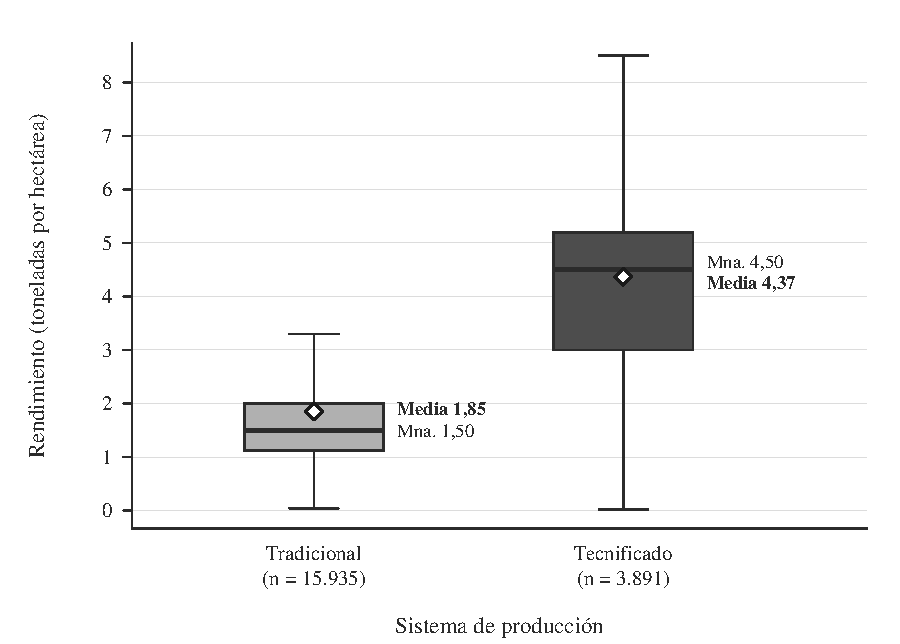
\includegraphics[width=0.9\linewidth]{../figuras/fig1_box_sistema.pdf}\end{center}

\apanota{$N = \Nfinal$ registros. El rombo blanco marca la media y la línea
gruesa la mediana; los bigotes llegan hasta 1{,}5 veces el rango
intercuartílico y se omiten los valores atípicos para no saturar el panel.
Elaboración propia con R a partir de UPRA (2025).}
\end{bloque}

\vspace{14pt}

\begin{bloque}
\apafigura{2}{Tres estimaciones de la brecha de rendimiento, con su intervalo de confianza del 95\,\%}

\begin{center}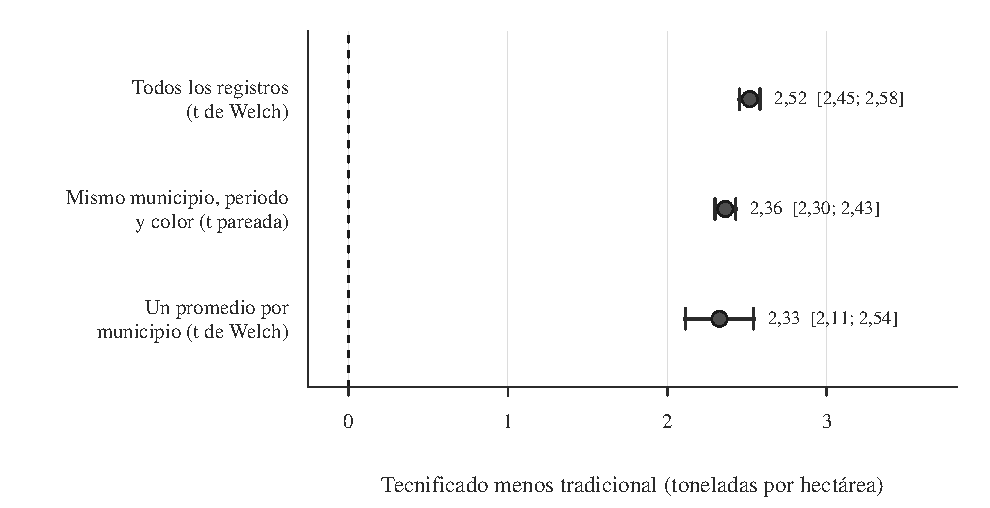
\includegraphics[width=\linewidth]{../figuras/fig2_ic_brecha.pdf}\end{center}

\apanota{El punto es la diferencia estimada y la barra, el intervalo de
confianza. La línea discontinua marca la ausencia de diferencia. Elaboración
propia con R a partir de UPRA (2025).}
\end{bloque}

\newpage

\begin{bloque}
\apafigura{3}{Porcentaje de registros con pérdida de área según el sistema de producción, con su intervalo de confianza del 95\,\%}

\begin{center}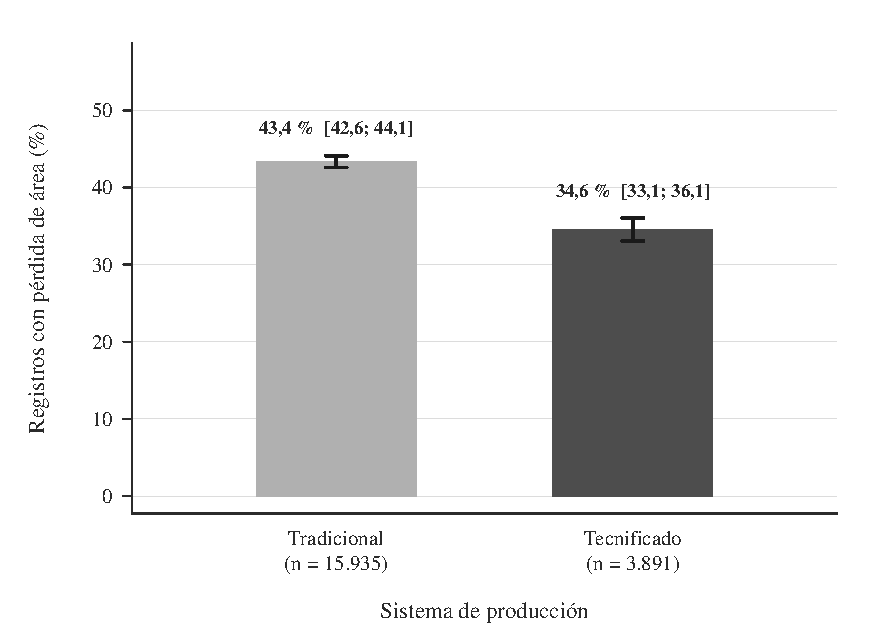
\includegraphics[width=0.8\linewidth]{../figuras/fig3_ic_perdida.pdf}\end{center}

\apanota{Hay pérdida de área cuando el área cosechada es menor que la
sembrada. Los porcentajes se calculan dentro de cada sistema. Elaboración
propia con R a partir de UPRA (2025).}
\end{bloque}

\vspace{14pt}

\begin{bloque}
\apafigura{4}{Área sembrada y producción de cada registro, con las rectas de regresión ajustadas}

\begin{center}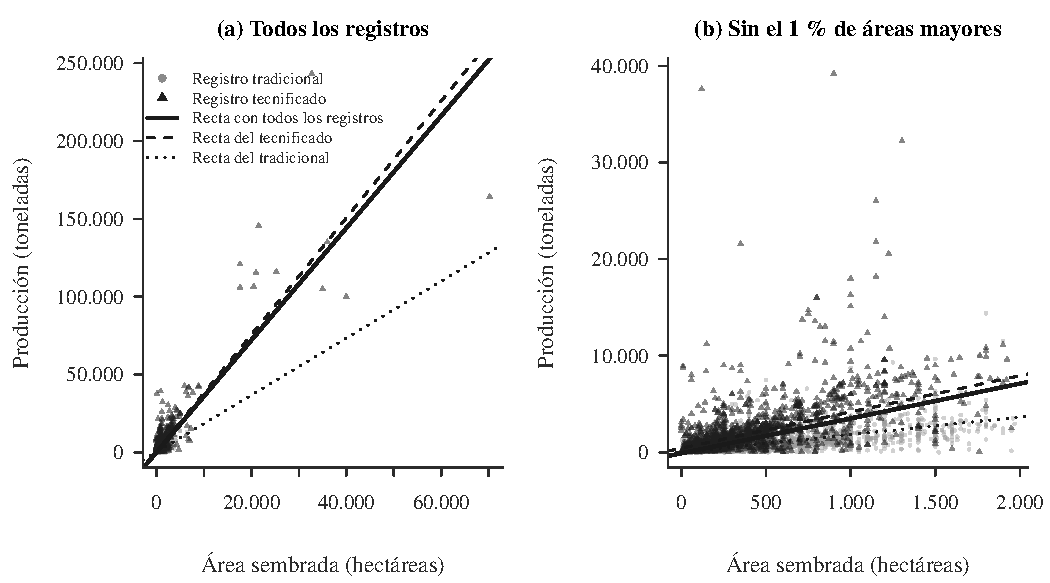
\includegraphics[width=\linewidth]{../figuras/fig4_dispersion.pdf}\end{center}

\apanota{Panel a: todos los registros. Panel b: sin el 1\,\% de registros con
mayor área sembrada (más de \CorteArea{}~ha), para ver la nube principal; las
rectas son las mismas del panel a y corresponden a la Tabla~4. Elaboración
propia con R a partir de UPRA (2025).}
\end{bloque}

\newpage

\begin{bloque}
\apafigura{5}{Diagnóstico de residuos del modelo con todos los registros}

\begin{center}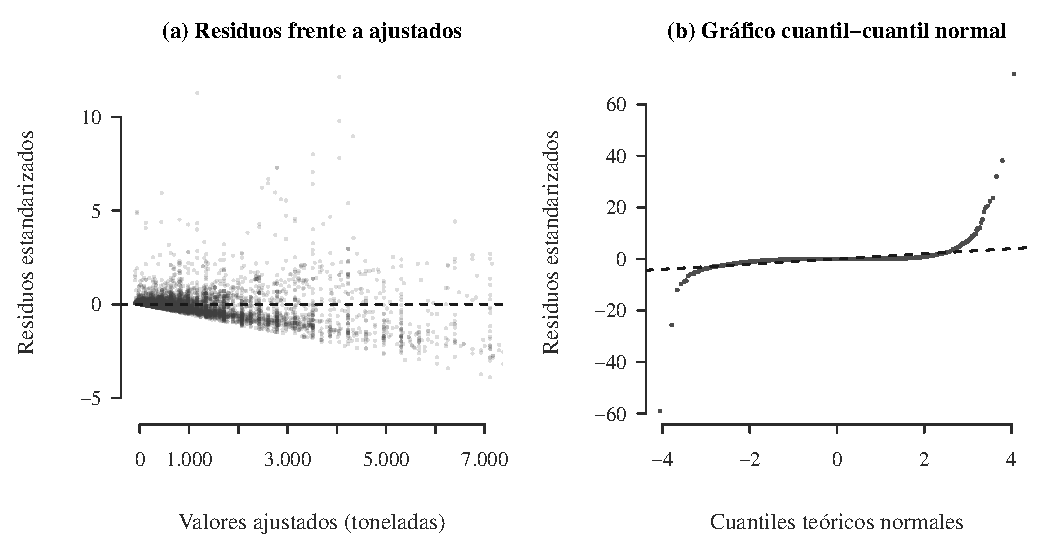
\includegraphics[width=\linewidth]{../figuras/fig5_residuos.pdf}\end{center}

\apanota{En el panel a se muestran los registros con valores ajustados por
debajo del percentil 99 y residuos entre los percentiles 0{,}05 y 99{,}95,
para que el eje sea legible; la línea discontinua marca el cero. En el
panel~b, la línea discontinua es la referencia normal. Elaboración propia con
R a partir de UPRA (2025).}
\end{bloque}

\vspace{14pt}

\begin{bloque}
\apafigura{6}{Pendiente de cada modelo de regresión, con sus intervalos de confianza del 95\,\% clásico y bootstrap}

\begin{center}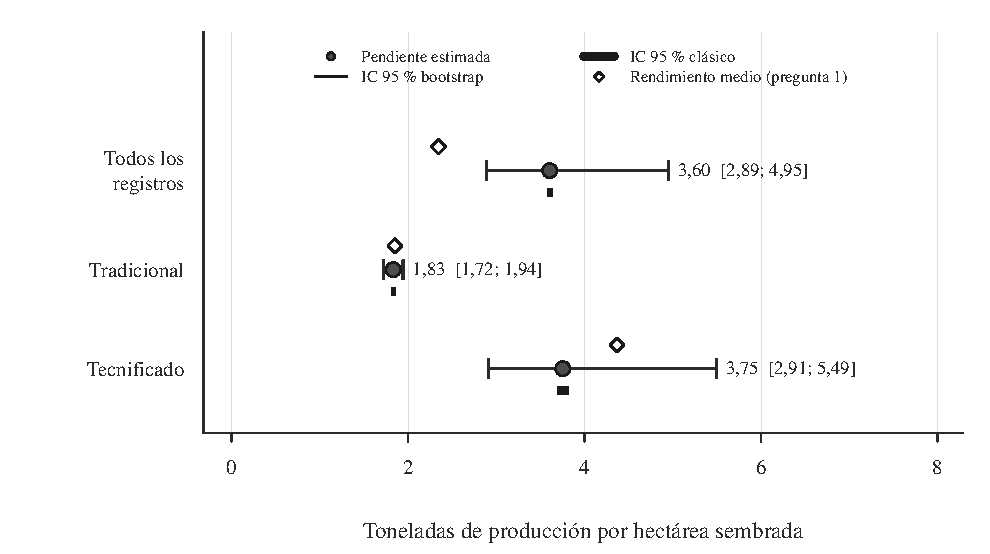
\includegraphics[width=0.95\linewidth]{../figuras/fig6_pendientes.pdf}\end{center}

\apanota{El punto es la pendiente estimada, en toneladas de producción por
hectárea sembrada; la línea delgada, el IC bootstrap percentil con \BBoot{}
remuestreos; la barra gruesa, el IC clásico, tan estrecho que casi se reduce a
un punto. El rombo es el rendimiento medio del grupo (pregunta~1). Elaboración
propia con R a partir de UPRA (2025).}
\end{bloque}

\end{document}
